\documentclass{report}

\usepackage{hyperref}

\usepackage{epstopdf}
\usepackage{amsmath}
\usepackage{amssymb}
\usepackage{subfig}
%\usepackage{multirow}
\usepackage[utf8]{inputenc}
\usepackage[T1]{fontenc}
\usepackage{standalone}
\usepackage{tikz}
\usepackage{tabularx}
\usepackage{float}
\usepackage[section]{placeins}

\graphicspath{{img/}}
\DeclareGraphicsExtensions{.pdf,.png,.jpg,.svg} %For pdflatex



\begin{document}


\begin{titlepage}
    \begin{center}
        \Huge
        \textbf{Przetwarzanie Obrazów Cyfrowych}
        \\ \vspace{1.5cm}
        \Large
        \textbf{Raport z ćwiczenia 1}        
    \end{center}
    \vspace{4.0cm}
    \Large
    Autor: \\
    Dawid Kania
    
\end{titlepage}


\section{Cel ćwiczenia}

Celem ćwiczenia jest zapoznanie się z różnymi formatami 
zapisu grafiki rastrowej wykorztywanymi przy tworzeniu dokumentów
cyfrowych, oraz stosowanymi w nich technikach kompresji


\section{Porównanie róźnych formatów zapisu}


Porównując poszczególne formaty zapisu możemy dostrzec że
w przypadku obrazów syntetycznych takich jak rzuty ekranu
metody kompresji (jpg i jp2) wprowadzają do obrazu nieprzyjemny szum. 
Ponadto rozmiar plików jest większy niż plików zapisanych metodami bezstratnymi (png i gif).

W przypadku rzeczywistych zdjęć różnice dla niewprawnego oka są
ledwo zauważalne. Rozmiar obrazów skompresowanych metodami stratnymi jest znacznie mniejszy
niż zdjęć zapisanych w formatach bezstratnych.

Metody bezstratne najlepiej stosować dla obrazów syntetycznych takich jak
wykresy, grafy i zrzuty ekranów gdzie szum wprowadzany przez stratne metody 
kompresji może być wyrażnie zauważalny.

Metody stratnej kompresji najlepiej stosować w przypadku zdjęć rzeczywistych
gdzie szum z oryginalnego zdjęcia jest trudny do rozróżnienia od szumu wprowadzanego
przez metody kompresji










\newcommand{\ww}{0.32}


\begin{figure}[H]
    \captionsetup[subfloat]{position=bottom,labelformat=empty} %można usunąć labelformat wówczas będzie label a), b), c) plus "opis"
    \subfloat[ PNG         \\  PSNR = Inf     \\ size = 231.959kB   ]{
\includegraphics[   width=\ww\linewidth]{../convertedImg/T1_4/c_1image.png.png       }} \hfill%
    \subfloat[ GIF         \\  PSNR = Inf     \\ size = 291.8145kB  ]{
\includegraphics[   width=\ww\linewidth]{../convertedImg/T1_4/c_2image.gif.png       }} \hfill% wypełnenie
    \subfloat[ JPG  q=80   \\  PSNR = 20.2377 \\ size = 116.3135kB  ]{
\includegraphics[   width=\ww\linewidth]{../convertedImg/T1_4/c_3image_Q80.jpg.png   }} \\ %nowa linia
    \subfloat[ JPG  q=50   \\  PSNR = 19.2892 \\ size = 66.5068kB   ]{
\includegraphics[   width=\ww\linewidth]{../convertedImg/T1_4/c_4image_Q50.jpg.png   }} \hfill%
    \subfloat[ JP2  q=30   \\  PSNR = 18.6797 \\ size = 24.9902kB   ]{
\includegraphics[   width=\ww\linewidth]{../convertedImg/T1_4/c_5image_Q30.jp2.png   }} \hfill%
    \subfloat[ JP2  q=20   \\  PSNR = 19.6769 \\ size = 37.9102kB   ]{
\includegraphics[   width=\ww\linewidth]{../convertedImg/T1_4/c_6image_Q20.jp2.png   }} 
    \caption{porównanie jakości różnych metod kompresji obrazu} %
    \label{fig:fig1}
\end{figure}



\begin{figure}
    \captionsetup[subfloat]{position=bottom,labelformat=empty} %można usunąć labelformat wówczas będzie label a), b), c) plus "opis"
    \subfloat[ PNG         \\  PSNR = Inf     \\ size = 168.3457kB ]{
\includegraphics[  width=\ww\linewidth]{../convertedImg/T1_2/c_1image.png.png      }} \hfill%
    \subfloat[ GIF         \\  PSNR = Inf     \\ size = 187.7178kB ]{
\includegraphics[  width=\ww\linewidth]{../convertedImg/T1_2/c_2image.gif.png      }} \hfill% wypełnenie
    \subfloat[ JPG  q=80   \\  PSNR = 31.864  \\ size = 68.9824kB  ]{
\includegraphics[  width=\ww\linewidth]{../convertedImg/T1_2/c_3image_Q80.jpg.png  }} \\ %nowa linia
    \subfloat[ JPG  q=50   \\  PSNR = 29.6045 \\ size = 39.0938kB  ]{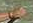
\includegraphics[  width=\ww\linewidth]{../convertedImg/T1_2/c_4image_Q50.jpg.png  }} \hfill%
    \subfloat[ JP2  q=30   \\  PSNR = 30.3839 \\ size = 25.1123kB  ]{
\includegraphics[  width=\ww\linewidth]{../convertedImg/T1_2/c_5image_Q30.jp2.png  }} \hfill%
    \subfloat[ JP2  q=20   \\  PSNR = 32.7683 \\ size = 37.9619kB  ]{
\includegraphics[  width=\ww\linewidth]{../convertedImg/T1_2/c_6image_Q20.jp2.png  }} 
    \caption{porównanie jakości różnych metod kompresji obrazu} %
    \label{fig:fig1}
\end{figure}



\begin{figure}
    \captionsetup[subfloat]{position=bottom,labelformat=empty} %można usunąć labelformat wówczas będzie label a), b), c) plus "opis"
    \subfloat[ PNG         \\  PSNR = Inf      \\  size = 243.2275kB ]{
\includegraphics[  width=\ww\linewidth]{../convertedImg/T1_3/c_1image.png.png       }} \hfill%
    \subfloat[ GIF         \\  PSNR = Inf      \\  size = 281.5684kB ]{
\includegraphics[  width=\ww\linewidth]{../convertedImg/T1_3/c_2image.gif.png       }} \hfill% wypełnenie
    \subfloat[ JPG  q=80   \\  PSNR = 27.9394  \\  size = 101.5342kB ]{
\includegraphics[  width=\ww\linewidth]{../convertedImg/T1_3/c_3image_Q80.jpg.png   }} \\ %nowa linia
    \subfloat[ JPG  q=50   \\  PSNR = 26.8454  \\  size = 56.9834kB  ]{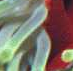
\includegraphics[  width=\ww\linewidth]{../convertedImg/T1_3/c_4image_Q50.jpg.png   }} \hfill%
    \subfloat[ JP2  q=30   \\  PSNR = 27.8981  \\  size = 32.7783kB  ]{
\includegraphics[  width=\ww\linewidth]{../convertedImg/T1_3/c_5image_Q30.jp2.png   }} \hfill%
    \subfloat[ JP2  q=20   \\  PSNR = 30.002   \\  size = 49.3682kB  ]{
\includegraphics[  width=\ww\linewidth]{../convertedImg/T1_3/c_6image_Q20.jp2.png   }} 
    \caption{porównanie jakości różnych metod kompresji obrazu} %
    \label{fig:fig1}
\end{figure}



\begin{figure}
    \captionsetup[subfloat]{position=bottom,labelformat=empty} %można usunąć labelformat wówczas będzie label a), b), c) plus "opis"
    \subfloat[ PNG         \\ PSNR = Inf     \\ size = 4.7705kB  ]{
\includegraphics[  width=\ww\linewidth]{../convertedImg/T1_s2/c_1image.png.png       }} \hfill%
    \subfloat[ GIF         \\ PSNR = Inf     \\ size = 6.9268kB  ]{
\includegraphics[  width=\ww\linewidth]{../convertedImg/T1_s2/c_2image.gif.png       }} \hfill% wypełnenie
    \subfloat[ JPG  q=80   \\ PSNR = 31.8698 \\ size = 20.0312kB ]{
\includegraphics[  width=\ww\linewidth]{../convertedImg/T1_s2/c_3image_Q80.jpg.png   }} \\ %nowa linia
    \subfloat[ JPG  q=50   \\ PSNR = 27.6401 \\ size = 13.8467kB ]{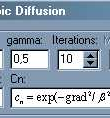
\includegraphics[  width=\ww\linewidth]{../convertedImg/T1_s2/c_4image_Q50.jpg.png   }} \hfill%
    \subfloat[ JP2  q=30   \\ PSNR = 27.5802 \\ size = 6.6826kB  ]{
\includegraphics[  width=\ww\linewidth]{../convertedImg/T1_s2/c_5image_Q30.jp2.png   }} \hfill%
    \subfloat[ JP2  q=20   \\ PSNR = 31.4605 \\ size = 9.9883kB  ]{
\includegraphics[  width=\ww\linewidth]{../convertedImg/T1_s2/c_6image_Q20.jp2.png   }} 
    \caption{porównanie jakości różnych metod kompresji obrazu} %
    \label{fig:fig1}
\end{figure}



\begin{figure}
    \captionsetup[subfloat]{position=bottom,labelformat=empty} %można usunąć labelformat wówczas będzie label a), b), c) plus "opis"
    \subfloat[ PNG         \\  PSNR = Inf     \\ size = 229.3359kB ]{
\includegraphics[  width=\ww\linewidth]{../convertedImg/T2_10/c_1image.png.png       }} \hfill%
    \subfloat[ GIF         \\  PSNR = Inf     \\ size = 271.9805kB ]{
\includegraphics[  width=\ww\linewidth]{../convertedImg/T2_10/c_2image.gif.png       }} \hfill% wypełnenie
    \subfloat[ JPG  q=80   \\  PSNR = 34.4813 \\ size = 64.9746kB  ]{
\includegraphics[  width=\ww\linewidth]{../convertedImg/T2_10/c_3image_Q80.jpg.png   }} \\ %nowa linia
    \subfloat[ JPG  q=50   \\  PSNR = 32.9163 \\ size = 35.4814kB  ]{
\includegraphics[  width=\ww\linewidth]{../convertedImg/T2_10/c_4image_Q50.jpg.png   }} \hfill%
    \subfloat[ JP2  q=30   \\  PSNR = 40.3495 \\ size = 42.7754kB  ]{
\includegraphics[  width=\ww\linewidth]{../convertedImg/T2_10/c_5image_Q30.jp2.png   }} \hfill%
    \subfloat[ JP2  q=20   \\  PSNR = 42.9683 \\ size = 64.3818kB  ]{
\includegraphics[  width=\ww\linewidth]{../convertedImg/T2_10/c_6image_Q20.jp2.png   }} 
    \caption{porównanie jakości różnych metod kompresji obrazu} %
    \label{fig:fig1}
\end{figure}



\begin{figure}
    \captionsetup[subfloat]{position=bottom,labelformat=empty} %można usunąć labelformat wówczas będzie label a), b), c) plus "opis"
    \subfloat[ PNG         \\ PSNR = 40.3649 \\ size = 85.5781kB ]{
\includegraphics[ width=\ww\linewidth]{../convertedImg/T3_1/c_1image.png.png       }} \hfill%
    \subfloat[ GIF         \\ PSNR = 40.3649 \\ size = 99.9502kB ]{
\includegraphics[ width=\ww\linewidth]{../convertedImg/T3_1/c_2image.gif.png       }} \hfill% wypełnenie
    \subfloat[ JPG  q=80   \\ PSNR = 34.7193 \\ size = 22.9365kB ]{
\includegraphics[ width=\ww\linewidth]{../convertedImg/T3_1/c_3image_Q80.jpg.png   }} \\ %nowa linia
    \subfloat[ JPG  q=50   \\ PSNR = 32.5026 \\ size = 13.3271kB ]{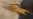
\includegraphics[ width=\ww\linewidth]{../convertedImg/T3_1/c_4image_Q50.jpg.png   }} \hfill%
    \subfloat[ JP2  q=30   \\ PSNR = 38.1796 \\ size = 23.8711kB ]{
\includegraphics[ width=\ww\linewidth]{../convertedImg/T3_1/c_5image_Q30.jp2.png   }} \hfill%
    \subfloat[ JP2  q=20   \\ PSNR = 41.1088 \\ size = 35.9658kB ]{
\includegraphics[ width=\ww\linewidth]{../convertedImg/T3_1/c_6image_Q20.jp2.png   }} 
    \caption{porównanie jakości różnych metod kompresji obrazu} %
    \label{fig:fig1}
\end{figure}


% -------------------------------------------------------------------------------------------
% -------------------------------------------------------------------------------------------
% -------------------------------------------------------------------------------------------


\section{Porównanie efektywności stratnych metod kompresji}


Na poniższych wykresach widać ze im większy stopień kompresji 
(im mniejsza jakość kompresji)
tym mniejszy rozmiar plików ale też tym mniejsza wartość wskaźnika PNSR 
(im mniejszy tym gorszej jakości kompresja)





\renewcommand{\ww}{0.16}

\begin{figure}
    \captionsetup[subfloat]{position=bottom,labelformat=empty} %można usunąć labelformat wówczas będzie label a), b), c) plus "opis"
    
    \subfloat[ Q=0    \\ size=8.66 kB    \\  ]{
\includegraphics[ width=\ww\linewidth]{../convertedImg2/jpg/000img.jpg.png   }} \hfill%
    \subfloat[ Q=5    \\ size=11.35 kB   \\  ]{
\includegraphics[ width=\ww\linewidth]{../convertedImg2/jpg/005img.jpg.png   }} \hfill%
    \subfloat[ Q=10   \\ size=17.24 kB   \\  ]{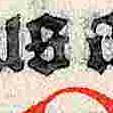
\includegraphics[ width=\ww\linewidth]{../convertedImg2/jpg/010img.jpg.png   }} \hfill% wypełnenie
    \subfloat[ Q=20   \\ size=28.78 kB   \\  ]{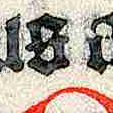
\includegraphics[ width=\ww\linewidth]{../convertedImg2/jpg/020img.jpg.png   }} \hfill
    \subfloat[ Q=30   \\ size=38.36 kB   \\  ]{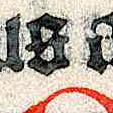
\includegraphics[ width=\ww\linewidth]{../convertedImg2/jpg/030img.jpg.png   }} \hfill%
    \subfloat[ Q=40   \\ size=46.20 kB   \\  ]{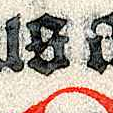
\includegraphics[ width=\ww\linewidth]{../convertedImg2/jpg/040img.jpg.png   }} \\
    \subfloat[ Q=50   \\ size=53.48 kB   \\  ]{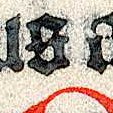
\includegraphics[ width=\ww\linewidth]{../convertedImg2/jpg/050img.jpg.png   }} \hfill%
    \subfloat[ Q=60   \\ size=61.28 kB   \\  ]{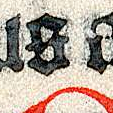
\includegraphics[ width=\ww\linewidth]{../convertedImg2/jpg/060img.jpg.png   }} \hfill% wypełnenie
    \subfloat[ Q=70   \\ size=73.24 kB   \\  ]{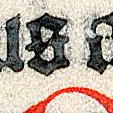
\includegraphics[ width=\ww\linewidth]{../convertedImg2/jpg/070img.jpg.png   }} \hfill
    \subfloat[ Q=80   \\ size=93.59 kB   \\  ]{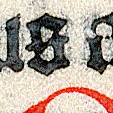
\includegraphics[ width=\ww\linewidth]{../convertedImg2/jpg/080img.jpg.png   }} \hfill%
    \subfloat[ Q=90   \\ size=141.37 kB  \\  ]{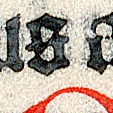
\includegraphics[ width=\ww\linewidth]{../convertedImg2/jpg/090img.jpg.png   }} \hfill
    \subfloat[ Q=100  \\ size=355.55 kB  \\  ]{
\includegraphics[ width=\ww\linewidth]{../convertedImg2/jpg/100img.jpg.png   }} \\%

    \caption{porównanie obrazów z różnym stopniem kompresji, obrazy zostały zapisane w formacie JPG} %
    \label{fig:fig1}
\end{figure}



\renewcommand{\ww}{0.5}
\begin{figure}
    \captionsetup[subfloat]{position=bottom,labelformat=empty} %można usunąć labelformat wówczas będzie label a), b), c) plus "opis"
    
    \subfloat[  ]{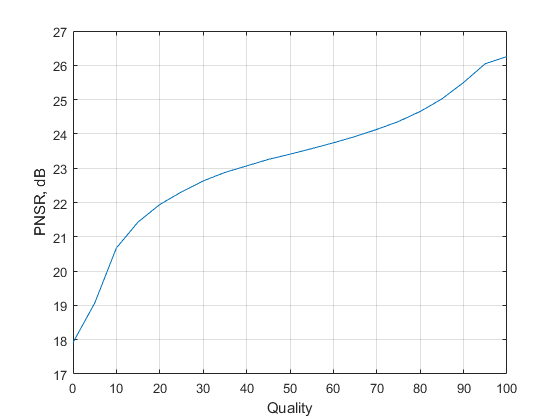
\includegraphics[ width=\ww\linewidth]{../matlab/pnsr_jpg.png   }} \hfill%
    \subfloat[  ]{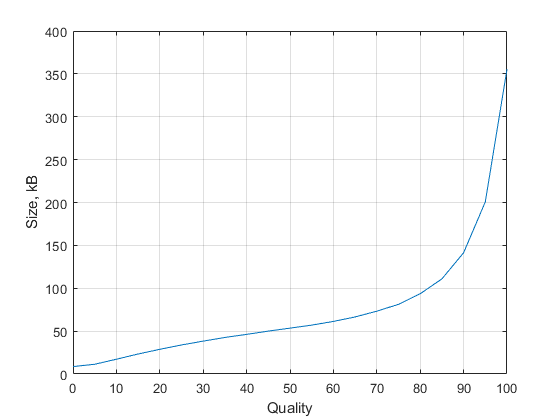
\includegraphics[ width=\ww\linewidth]{../matlab/size_jpg.png   }} \hfill%

    \caption{rozmiar pliku i wskaźnik jakości PNSR w zależności od stopnia kompresji dla formatu JPG} %
    \label{fig:fig1}
\end{figure}




\renewcommand{\ww}{0.5}
\begin{figure}

    \includegraphics[]{../matlab/size_pnsr_jpg.png   }
    \centering

    \caption{zależność wskażnika PNSR od rozmiaru pliku} %
    \label{fig:fig1}
\end{figure}






\renewcommand{\ww}{0.16}

\begin{figure}
    \captionsetup[subfloat]{position=bottom,labelformat=empty} %można usunąć labelformat wówczas będzie label a), b), c) plus "opis"
    
    \subfloat[ Q = 1    \\  size=558.35 kB \\ ]{\includegraphics[ width=\ww\linewidth]{../convertedImg2/jp2/001img.jp2.png   }} \hfill%
    \subfloat[ Q = 2    \\  size=383.41 kB \\ ]{\includegraphics[ width=\ww\linewidth]{../convertedImg2/jp2/002img.jp2.png   }} \hfill%
    \subfloat[ Q = 4    \\  size=191.39 kB \\ ]{\includegraphics[ width=\ww\linewidth]{../convertedImg2/jp2/004img.jp2.png   }} \hfill% wypełnenie
    \subfloat[ Q = 7    \\  size=109.18 kB \\ ]{\includegraphics[ width=\ww\linewidth]{../convertedImg2/jp2/007img.jp2.png   }} \hfill
    \subfloat[ Q = 12   \\  size=63.52 kB  \\ ]{\includegraphics[ width=\ww\linewidth]{../convertedImg2/jp2/012img.jp2.png   }} \hfill%
    \subfloat[ Q = 23   \\  size=32.92 kB  \\ ]{\includegraphics[ width=\ww\linewidth]{../convertedImg2/jp2/023img.jp2.png   }} \\
    \subfloat[ Q = 43   \\  size=17.41 kB  \\ ]{\includegraphics[ width=\ww\linewidth]{../convertedImg2/jp2/043img.jp2.png   }} \hfill%
    \subfloat[ Q = 81   \\  size=9.27 kB   \\ ]{\includegraphics[ width=\ww\linewidth]{../convertedImg2/jp2/081img.jp2.png   }} \hfill% wypełnenie
    \subfloat[ Q = 152  \\  size=4.82 kB   \\ ]{\includegraphics[ width=\ww\linewidth]{../convertedImg2/jp2/152img.jp2.png   }} \hfill
    \subfloat[ Q = 285  \\  size=2.77 kB   \\ ]{\includegraphics[ width=\ww\linewidth]{../convertedImg2/jp2/285img.jp2.png   }} \hfill%
    \subfloat[ Q = 534  \\  size=1.52 kB   \\ ]{\includegraphics[ width=\ww\linewidth]{../convertedImg2/jp2/534img.jp2.png   }} \hfill
    \subfloat[ Q = 1000 \\  size=0.85 kB   \\ ]{\includegraphics[ width=\ww\linewidth]{../convertedImg2/jp2/1000img.jp2.png   }} \\%

    \caption{porównanie obrazów z różnym stopniem kompresji, obrazy zostały zapisane w formacie JP2} %
    \label{fig:fig1}
\end{figure}



\renewcommand{\ww}{0.5}
\begin{figure}
    \captionsetup[subfloat]{position=bottom,labelformat=empty} %można usunąć labelformat wówczas będzie label a), b), c) plus "opis"
    
    \subfloat[  ]{\includegraphics[ width=\ww\linewidth]{../matlab/pnsr_jp2.png   }} \hfill%
    \subfloat[  ]{\includegraphics[ width=\ww\linewidth]{../matlab/size_jp2.png   }} \hfill%

    \caption{rozmiar pliku i wskaźnik jakości PNSR w zależności od stopnia kompresji dla formatu JP2} %
    \label{fig:fig1}
\end{figure}


\renewcommand{\ww}{0.5}
\begin{figure}

    \includegraphics[]{../matlab/size_pnsr_jp2.png   }
    \centering

    \caption{zależność wskażnika PNSR od rozmiaru pliku} %
    \label{fig:fig1}
\end{figure}



\end{document}